\documentclass[12pt]{article}
\usepackage[utf8]{inputenc}
\usepackage{amsmath,amsfonts}
\usepackage{graphicx}
\usepackage{algorithm}
\usepackage{subcaption}

\DeclareMathOperator*{\argmin}{arg\,min}
\providecommand{\m}[1]{\mathbf{#1}}
\providecommand{\norm}[1]{\left\|#1\right\|}
\usepackage{abstract}
\renewcommand{\abstractname}{}    % clear the title
\renewcommand{\absnamepos}{empty} % originally center

\addtolength{\textheight}{1in}
\addtolength{\voffset}{-1in}

\setlength{\textwidth}{5in}
\begin{document}
\title{Auto Scaling Online Learning}
\author{Marco Tulio Ribeiro, Shrainik Jain}
\renewcommand{\today}{Mar 17, 2014}
\maketitle

\begin{abstract}
We propose a framework and algorithms for scaling online machine learning up
or down, according to demand, and the priorities of the system. Different
systems have different needs in terms of the cost assigned to machines, the cost
of a bad user experience, etc. In this project, we focus most on the part that
is general to auto scaling any application (and not only machine learning
algorithms), but propose a framework that takes some ML particularities into
account.
\end{abstract}


\section{Introduction}
Online machine learning algorithms operate on a single instance at a time. They
have become particularly popular in natural language processing and applications
with streaming data, including classification, ranking, etc
\cite{Bordes:2005:HSE:2130928.2130979,
Carvalho:2006:SOL:1150402.1150466, Dredze:2008:CLC:1390156.1390190}. Online
learning is particularly interesting in the scenarios where data keeps streaming
in, such as a web search engine doing advertisement placement. It is also
interesting for scenarios where the whole dataset is too large to fit in main
memory, as online learning only operates on a single example at a time.

A lot of tasks that use online learning have a particular structure that can be 
broken down into 2 major components: 1 - Learning a model from data, and 2 -
making predictions according to the model. Going back to the web search engine
scenario as an example: the system needs to make predictions for every user
doing a query - and must also learn from the feedback given by those users. We
call machines that make predictions \textbf{predictors}, and machines that learn
from the feedback \textbf{learners}.

This structure comes with multiple challenges. First, the 
the amount of data is always growing, so archiving it comes at a cost, both
because of storage constraints and computation constraints. A solution to this
is to just keep the current model in memory, and archive the rest in the
background. A second challenge is the
variable speed at which data streams in. Imagine a learning problem where in the
learning dataset is a live twitter stream for a hashtag. In this scenario the
rate at which the data comes in is a function of the popularity of the hashtag.
Finally, different applications have different costs for learning, and different
requirements for the latency of predictions.

The problem we tackled in this project is the problem of automatically
handling the resources needed for online learning. The ideal system would
allocate the resources necessary to keep the prediction latency acceptable,
while at the same time learning appropriately. Finally, the system would be able
to handle bursts (such as increase in demand) and different learning
requirements for different systems. Since online learning in a distributed
system is a research problem on its \cite{pserver1, pserver2}, we abstracted
this part from our work, and focused on some of the systems challenges.

Current works in auto-scaling\cite{Mao:2011:AMC:2063384.2063449,6008748} address
many of the issues we address in this report (such as load prediction, framing
the problem as a cost minimization problem, etc). However, one aspect that we
thought was lacking in current work (at least from the papers we read) is
dealing with node failures and uncertainty. We reformulate the cost function in
terms of expected cost, in order to account for uncertainty pertaining future
load predictions and node failures. Finally, we evaluate some baselines and our
proposed approach with simulated loads.

\section{Architecture}
\begin{figure}[h!]
\center
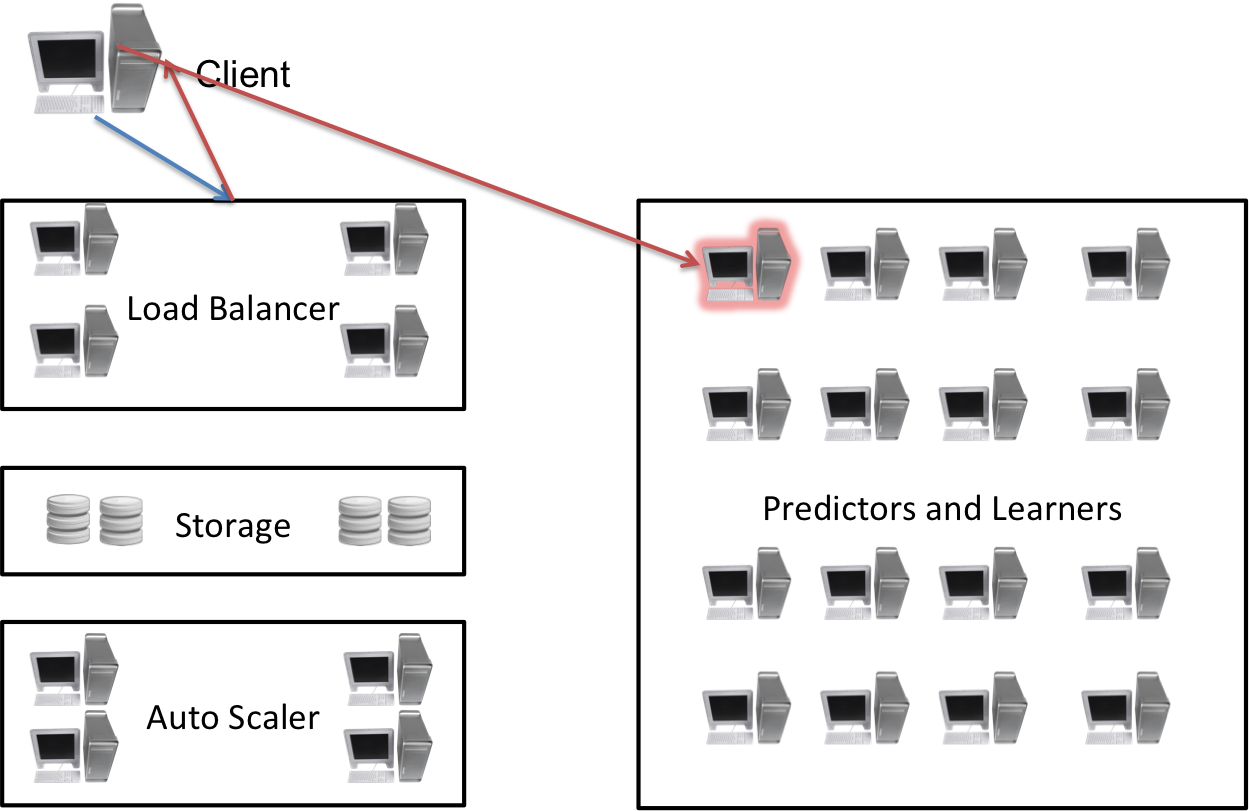
\includegraphics[width=1.0\textwidth]{architecture.png}
\caption{Architecture: Node asks the load balancer for a predictor, and then
asks the predictor for a prediction.}
\label{architecture}
\end{figure}

We assume an architecture similar to the one presented in Figure
\ref{architecture}. There is a set of nodes acting as a Load Balancer
(whose addresses are known to the clients of the machine learning service). When
a client needs a predictor or a learner, it first requests an a node from the
Load Balancer, and then it proceeds to make the request. In Figure
\ref{architecture}, the client got assigned the node in red.

The Load Balancer reads the state of the current system from some distributed,
reliable storage. The state is comprised of which nodes are up and acting as
learners or predictors, and a measure of the \textbf{power} of each node - that
is, how many requests each node can effectively handle in a time interval. This
allows for load balancing even when heterogeneous nodes are present.

The state of the current system is modified every so often by the set of nodes
denoted \textbf{Autoscaler} in Figure \ref{architecture}. The Autoscaler
periodically sends heartbeat messages to nodes and to the load balancer, and
tests the prediction / learning time. It also gets the status - i.e., the number
of requests served, eventual node failures, etc.  Finally, it then updates the
state in the distributed storage according to some policy. This architecture is
very straightforward, and can be used with commodity machines for handling a lot
of requests, while still being resilient to failures (depending of course on the
Autoscaler policy).

\section{Auto Scaling}
\subsection{Objective}
The problem of auto scaling online learning can be formulated as minimizing a
cost function over a sequence of time intervals. This function for each time
interval is presented in
Equation 1. 
\begin{equation}
cost = \alpha SLA + \beta P + \gamma LR + \delta L
\end{equation}
\textbf{SLA} is an indicator variable that is positive when a Service License
Agreement (SLA) is violated in the time interval in question. This SLA is
related to predictions, and can be defined as a threshold on the average time
per prediction, on the maximum time per prediction, etc. There is a cost
$\alpha$ associated with the SLA violation, that depends on the specific
application that depends on the system. A bad user experience due to slow
page loading on a search engine can be fatal to the success of the business,
while a slower prediction for some internal testing service can be less costly.
\textbf{P} denotes the number of predictors active in the time interval, while
$\beta$ is a measure of the cost of each predictor. \textbf{LR} is a measure of
the learning rate achieved by the machine learning algorithm. Some of the most
popular online learning algorithms, such as Stochastic Gradient Descent, have a
property that error $\epsilon$ decreases
linearly with the number of training examples
\cite{Nemirovski:2009:RSA:1654243.1654247}: that is, the relation is $O(1 /
\epsilon)$ , meaning that if training examples
are available, adding more learners would offset the training error, and thus
increase whatever measure of Learning Rate is being used - although probably not with
linear speedup \cite{pserver1, pserver2}.  $\textbf{L}$ denotes
the number of learners active in the time interval.

This objective formulation decouples learning from predicting, which brings
advantages and disadvantages. Usually, the processor / memory requirements for
learning and predicting are different - one would want a more powerful machine
for learning than for predicting. Decoupling also ensures that failures in
learners do not affect predictors, and vice versa. However, having learners and
predictors together could be interesting in that learning involves predicting,
and thus separating them creates the need to do predictions twice for the same
examples: once in the predictor and once in the learner. In this project, we
abstracted out the learning part, and focused on minimizing the first two terms
in Equation 1. This choice was made assuming that a fixed, small number of
learners would be sufficient for many applications, and that this number would
not need to be changed very often - in contrast to predictors, who would need to
be changed according to load.

\subsection{Load Prediction}
Ideally, we would employ a machine learning algorithm in order to predict the
load in each future time interval. Features that we would consider include:
\begin{enumerate}
\item Time of day: traffic in most applications have load patterns that are very
time-specific. Most people are sleeping at night, have a lunch break around the
middle of the day, etc.
\item Trends in other services by the same company: if Facebook sees an increase
in the number of users in the website at a particular time, it is more likely
that internal services that use machine learning will also see an increase.
\item Usual load pattern: certain applications have very predictable load
patterns. An internal service that always gets called in exponentially growing
bursts would be an example.
\item Trend in the last time interval(s): by measuring the load at smaller
intervals in the last time interval, one can build a ``load trend'' for the next
time interval.
\end{enumerate}
Since we used simulated data (we do not have access to such a rich dataset), we
employed the trend in the last time interval in order to predict future load, by
using traditional linear regression. In order to ensure a smoother decay (and
thus prevent SLA violations due to wrong predictions), we took the max between the upper limit
on a 95\% confidence interval on the linear regression and the number of
requests in the previous time interval as a prediction. Figure \ref{loadsss}
illustrates the behaviour of our predictions on simulated data. We assume that
we must predict the load at every minute, and collect the current load at every
5 seconds in order to build the trend line. The blue lines are the actual load,
while the green and yellow lines indicate the linear regression prediction and
the max we cited before, respectively. It is clear that the yellow line is more
``conservative'', and always stays on top of the actual load. This is what we
used for predicting loads in our experiments.

\begin{figure}[h!]
\centering
\begin{subfigure}{.6\textwidth}
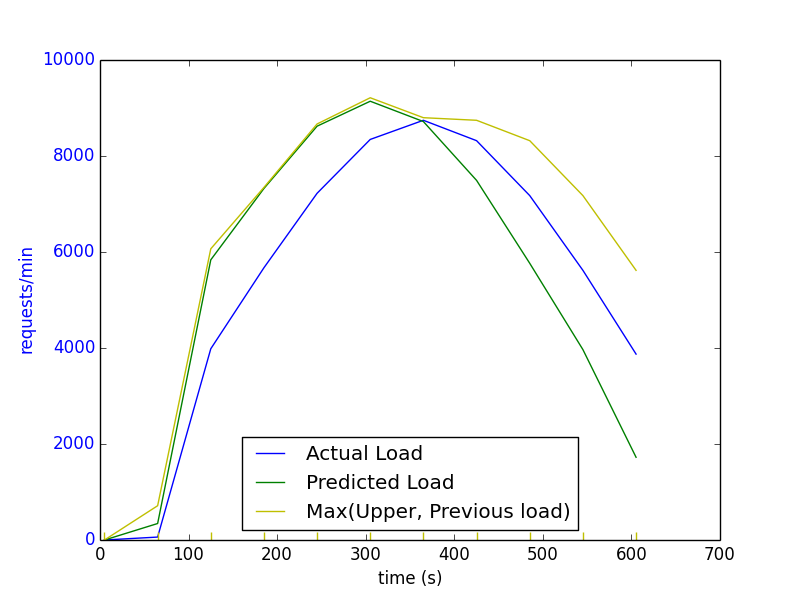
\includegraphics[width=\textwidth]{Smart182predictedVsActual.png}
\caption{Load Pattern 1}
\end{subfigure}
\begin{subfigure}{.6\textwidth}
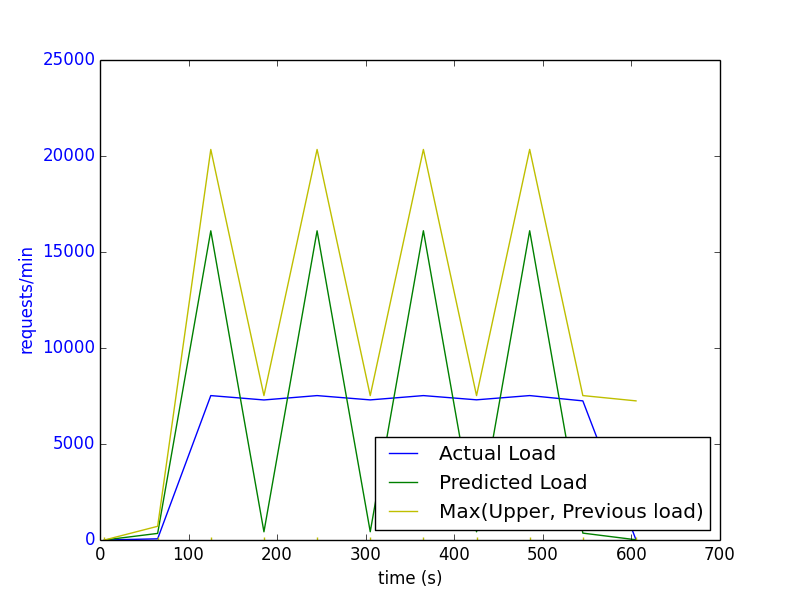
\includegraphics[width=\textwidth]{Smart282predictedVsActual.png}
\caption{Load Pattern 2}
\end{subfigure}
\begin{subfigure}{.6\textwidth}
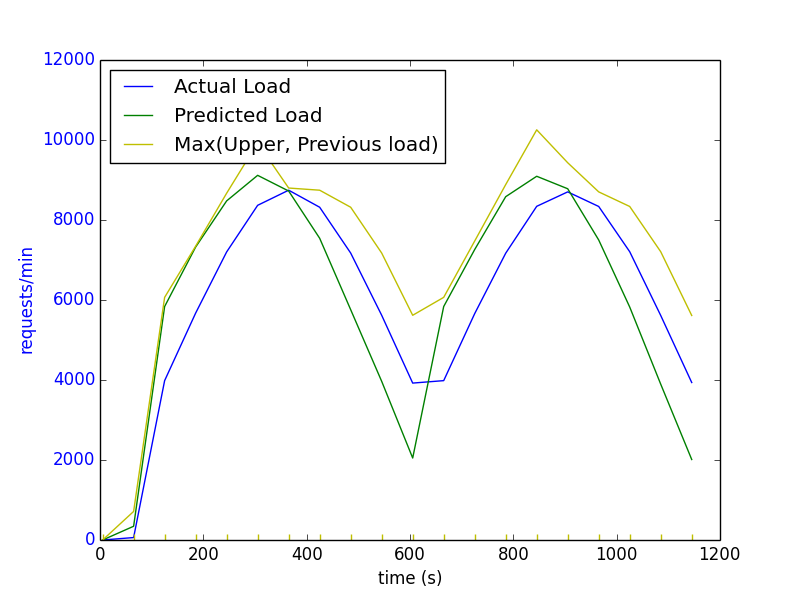
\includegraphics[width=\textwidth]{Smart382predictedVsActual.png}
\caption{Load Pattern 3}
\end{subfigure}
\caption{Predicted vs Actual load, different load patterns.}
\label{loadsss}
\end{figure}

\subsection{Strategies}
\bibliographystyle{plain}
\bibliography{references}

\end{document}
